\documentclass[12pt,a4paper,twoside,openright]{report}
\usepackage[pdfborder={0 0 0}]{hyperref}    % turns references into hyperlinks
\usepackage[margin=25mm]{geometry}  % adjusts page layout
\usepackage{graphicx}  % allows inclusion of PDF, PNG and JPG images
\usepackage{verbatim}
\usepackage{docmute}   % only needed to allow inclusion of proposal.tex
\usepackage[utf8]{inputenc}
\usepackage[english]{babel}
\usepackage{graphicx}
\usepackage{wrapfig}
\usepackage{float}

\raggedbottom                           % try to avoid widows and orphans
\sloppy
\clubpenalty1000%
\widowpenalty1000%

\renewcommand{\baselinestretch}{1.1}    % adjust line spacing to make
                                        % more readable

\begin{document}

\bibliographystyle{plain}

%%%%%%%%%%%%%%%%%%%%%%%%%%%%%%%%%%%%
%%%%%%%%%%%%%%% TITLE %%%%%%%%%%%%%%%%%
%%%%%%%%%%%%%%%%%%%%%%%%%%%%%%%%%%%%

\pagestyle{empty}

\rightline{\LARGE \textbf{Tudor Mihai Avram}}

\vspace*{60mm}
\begin{center}
	\Huge
	\textbf{Machine learning graph filtering} \\[5mm]
	Computer Science Tripos -- Part II \\[5mm]
	Homerton College \\[5mm]
	\today  % today's date
\end{center}

%%%%%%%%%%%%%%%%%%%%%%%%%%%%%%%%%%%%
%%%%%%%%%%%% PROFORMA %%%%%%%%%%%%%%%%
%%%%%%%%%%%%%%%%%%%%%%%%%%%%%%%%%%%%

\pagestyle{plain}

\chapter*{Proforma}

{\large
	\begin{tabular}{ll}
		Name:               & \bf Tudor Mihai Avram                     \\
		College:            & \bf Homerton College                    \\
		Project Title:      & \bf Machine learning graph filtering \\
		Examination:        & \bf Computer Science Tripos -- Part II, July 2018  \\
		Word Count:         & \bf 1\footnotemark[1] \\
		Project Originator: & Dr Ripduman Sohan                   \\
		Supervisor:         & Dr Lucian Carata                    \\ 
	\end{tabular}
}

\footnotetext[1]{This word count was computed
	by \texttt{detex dissertation.tex | tr -cd '0-9A-Za-z $\tt\backslash$n' | wc -w}
}

\section*{Original aims of the project}
\section*{Work completed}
\section*{Special Difficulties}

\newpage

\section*{Declaration}

%%%%%%%%%%%%%%%%%%%%%%%%%%%%%%%%%%%%
%%%%%%%% TABLE OF CONTENTS %%%%%%%%%%%%%
%%%%%%%%%%%%%%%%%%%%%%%%%%%%%%%%%%%%

\tableofcontents

%%%%%%%%%%%%%%%%%%%%%%%%%%%%%%%%%%%%
%%%%%%%%%%%% LIST OF FIGURES %%%%%%%%%%%%%
%%%%%%%%%%%%%%%%%%%%%%%%%%%%%%%%%%%%

\listoffigures

%%%%%%%%%%%%%%%%%%%%%%%%%%%%%%%%%%%%
%%%%%%%%%%%% LIST OF TABLES %%%%%%%%%%%%%
%%%%%%%%%%%%%%%%%%%%%%%%%%%%%%%%%%%%

\listoftables

%%%%%%%%%%%%%%%%%%%%%%%%%%%%%%%%%%%%
%%%%%%%%%%%%  INTRODUCTION %%%%%%%%%%%%%
%%%%%%%%%%%%%%%%%%%%%%%%%%%%%%%%%%%%

\chapter{Introduction}

This dissertation proposes an extension of the CADETS user interface (see \ref{1.1.1}). It uses Machine Learning techniques in order to filter a graph describing OS-level abstractions (i.e. to decide which nodes should be displayed to the analyst for further review). In order to achieve this, I implemented a number of different algorithms, in order to decide which would be applicable in this context. I also implemented one extensions: a server infrastructure that facilitates communications between the classifier and the client.

\section{Aims \& Motivation}  \label{1.1}
Analysing event logs of a distributed system in order to identify actionable security information and hence to act accordingly in order to improve a system's security has always been a desirable goal for both research and industry. The availability of cheap data storage has facilitated such large scale logs collection, in the order of several terabytes of data. This makes manual log review an unfeasible task. 

\subsection{Overview of CADETS UI}\label{1.1.1}
CADETS UI is a cybersecurity logs analysis tool developed as part of the CADETS and OPUS research projects. It displays logs as a network, emphasising the relationships between events. It is the analyst's task to explore this network in order to identify potentially malicious nodes.
\\ \\
In order to provide the analyst with comprehensive data from which he can infer useful information, the network will have a large number of nodes. This makes exploring the entire dataset a very difficult task for a human.  For example, tracing two machines for 7 minutes can produce as many as 6000 nodes in the network.  As the number of machines and the time interval we do tracing on increase, this number will become considerably larger, making analyst's job very difficult. 
\begin{figure}[H]
	\caption{\bf Snapshot of CADETS UI}
	\centering
	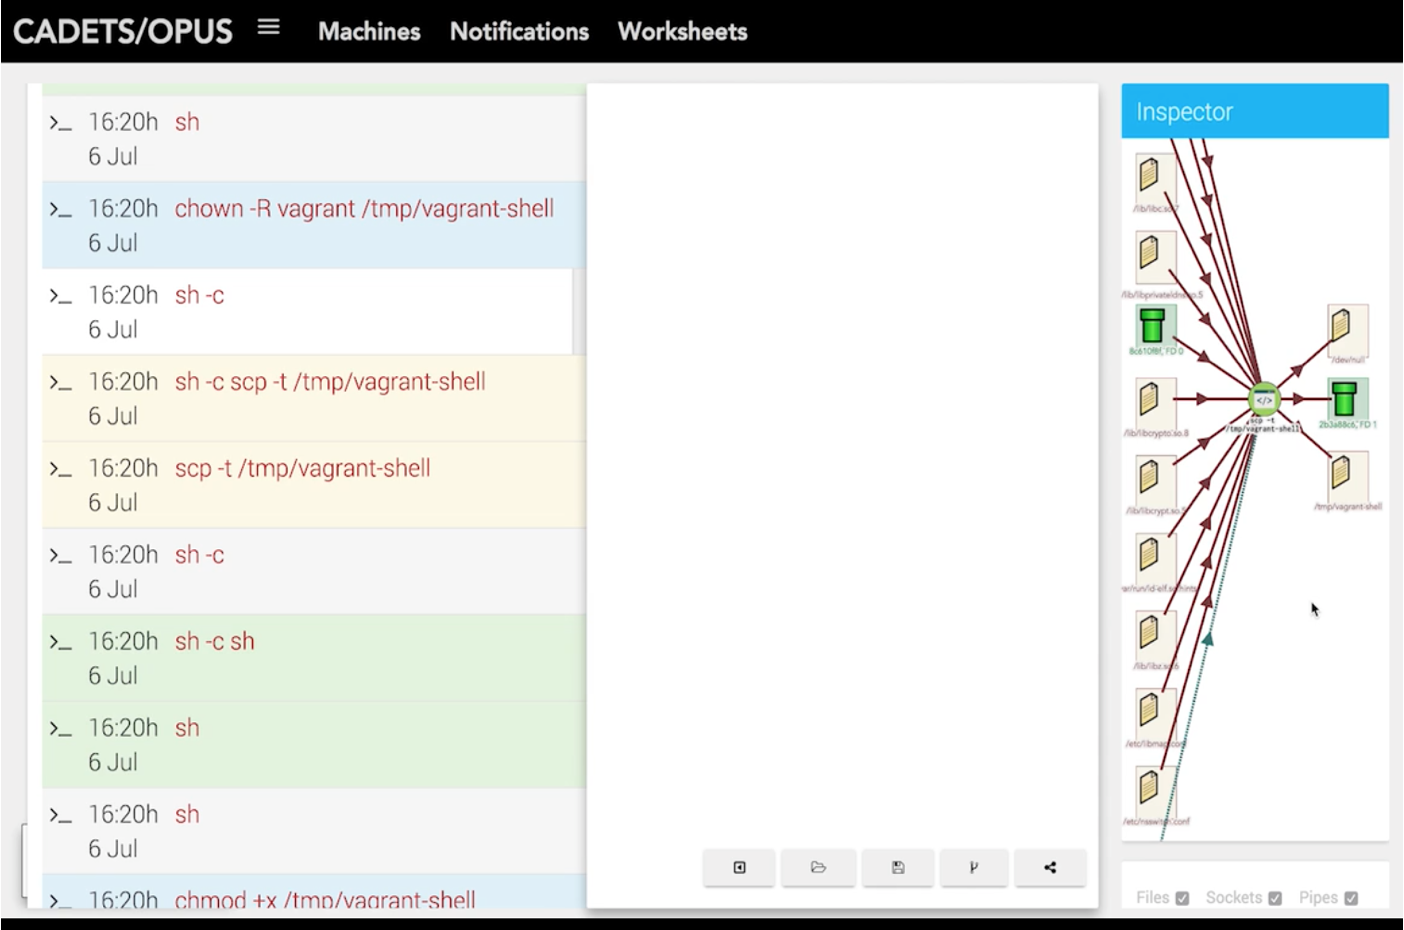
\includegraphics[width=0.7\textwidth]{graphics/CADETS}
\end{figure}

\subsection{Aims of the project}
In general, the number of nodes that are of interest to the analyst is significantly lower than the number of nodes that are not. Therefore, the aim of this project is to build a tool that would meliorate the analyst's experience by reducing the number of nodes he would have to cover. In order to achieve this, I will use a machine learning model that would classify nodes into nodes that are of interest and nodes that are not of interest, respectively. The training data used by this model is constructed based on a set of pre-defined ground-truths. 

\section{Overview of the architecture}
The communications between the CADETS user interface and the machine learning model is facilitated by a REST API. For performance purposes, it also uses a local cache of previous classifications. 
\\ \\ 
When it receives a request from the client, the server would first check the local cache. If it can find the classification result for that node, then it just returns the cached value to the client.
\begin{figure}[H]
	\caption{\bf Overview of the project's architecture}
	\centering
	\includegraphics[width=0.8\textwidth]{graphics/overview}
\end{figure}
If the result is not in the cache or if the cached value expired, it runs the machine learning model in order to classify that specific node. Once the classification is done, the result is stored in the local cache and returned to the client. 

\section{Related work}
Cyber security has always been a major concern in Computer Science, both in industry and in research. With the recent interest shown in Artificial Intelligence and Machine Learning, there has been an increasing number of tools that use related methodologies to identify malicious behaviour. This section will address some of these tools. 

\subsection{Clearcut}
Clearcut\footnotemark[1] is an open source tool that uses Machine Learning techniques for incident detection. It takes HTTP proxy logs as input and filters them for manual review, in order to aid the analyst in reviewing them. 
\\ \\ 
The algorithm used in this case is Random Forrest Classification, which essentially means having multiple decision trees in training and returning the class corresponding to the mode of the classes returned by them. 

\footnotetext[1]{\textbf{\url{https://github.com/DavidJBianco/Clearcut}}}

\subsection{Polonium}
Polonium is a scalable and effective technology that uses graph mining for malware detection. The tool uses a bipartite graph that consists of machines and files as its training data. It uses the Belief Propagation algorithm, which, at a high level, infers the label of a node from some prior knowledge about the node and from the node's neighbours. This is done through iterative message passing between all pairs of nodes $(u, v)$ in the graph. 
\\ \\
Although the problem statement is similar to that my project tries to address, the algorithm used here is not applicable in my case, because it requires a very large dataset (Polonium uses a graph with ~1 billion nodes). It also requires a pre-computed \textit{machine reputation} score that in this case is calculated using a proprietary formula of Symantec\footnotemark[2], the company that produced the tool. 

\footnotetext[2]{\textbf{\url{https://www.symantec.com/}}}

\section{Licence} 
The code is publicly available as an open-source project on GitHub\footnotemark[3], under an APACHE 2.0 licence\footnotemark[4]. 


\footnotetext[3]{\textbf{\url{https://github.com/a96tudor/Part2Project}}}
\footnotetext[4]{\textbf{\url{https://www.apache.org/licenses/LICENSE-2.0}}}
\end{document}